%%%%%%%%%%% System Analysis and Design %%%%%%%%%%%%%%%%%
\chapter{System Analysis and Design} \label{ch3_design}
\markboth{System Analysis and Design}{System Analysis and Design}

Following the theoretical exploration of distributed ledger technologies in Chapter \ref{ch2_theoretical_framework}, this chapter details the comprehensive design of the educational blockchain artifact. The primary challenge in designing this system lies in balancing \textbf{production-grade functionality} (networking, cryptography, consensus) with \textbf{educational clarity}.

The system is architected using a modular "Glass-Box" design philosophy, ensuring that complex components such as the consensus engine or the networking layer can be isolated, inspected, and modified by students without compromising the integrity of the entire system.

\section{Requirement Analysis} \label{ch3_requirements}

The requirements for the system were derived from the pedagogical needs of the curriculum defined in this research. They are categorized into Functional Requirements (system capabilities) and Non-Functional Requirements (system qualities) \cite{sommerville2011software}.

\subsection{Functional Requirements}
To serve as a viable laboratory platform, the system must support the following core operations:

\begin{enumerate}
    \item \textbf{Peer-to-Peer Networking:} The system must autonomously discover peers and propagate messages (blocks and transactions) using a TCP-based gossip protocol \cite{coulouris2011distributed}.
    \item \textbf{Pluggable Consensus:} The architecture must allow for the "Hot-Swapping" of consensus algorithms (e.g., switching from Proof of Stake to Proof of Work) via configuration, without code rewriting.
    \item \textbf{State Management:} The system must maintain a persistent ledger state (UTXO or Account-based) and resolve forks automatically using the "Longest Chain" rule.
    \item \textbf{Visual Observability:} A RESTful API must expose internal metrics (mempool size, peer count, last hash) to a frontend Blockchain Explorer.
\end{enumerate}

\subsection{Non-Functional Requirements}
\begin{enumerate}
    \item \textbf{Modularity:} The codebase must adhere to the Separation of Concerns principle. The networking logic must be decoupled from the business logic.
    \item \textbf{Deployability:} The system must be containerizable using Docker to ensure consistent behavior across different student operating systems.
    \item \textbf{Readability:} As an educational tool, the source code must prioritize clarity over micro-optimizations, utilizing Python's explicit syntax \cite{guzdial2004programming}.
\end{enumerate}

\section{System Architecture} \label{ch3_architecture}

The system adopts a \textbf{Layered Architecture} pattern, dividing the node into three distinct layers: The Networking Layer, the Core Blockchain Layer, and the Application Interface Layer.

% \begin{figure}[h]
%     \centering
%     % Placeholder for the Diagram
%     \includegraphics[width=0.8\textwidth]{figures/system_architecture_diagram.png}
%     \caption{High-Level Layered Architecture of the Blockchain Node}
%     \label{fig:arch_diagram}
% \end{figure}

\subsection{The Networking Layer (P2P)}
This layer handles the raw TCP socket connections. It implements a custom message handler that serializes Python objects into JSON payloads for transmission. By abstracting the socket logic here, the upper layers can simply invoke `broadcast(message)` without managing connection states.

\subsection{The Core Blockchain Layer}
This is the central engine of the system. It contains the data structures (Block, Transaction) and the validation logic. Crucially, this layer utilizes the **Strategy Design Pattern** to manage consensus. The `Blockchain` class does not implement mining logic directly; instead, it holds a reference to an `IConsensus` interface, allowing the implementation (PoW or PoS) to be injected at runtime \cite{gamma1995design}.

\subsection{The Application Interface (API)}
Built using \textbf{FastAPI}, this layer exposes the node's internal state to the external world. It serves as the bridge for the "Blockchain Explorer" and allows students to manually trigger actions (e.g., `POST /connect\_peer`) during laboratory exercises.

\section{Detailed Component Design} \label{ch3_detailed_design}

\subsection{Class Design and Relationships}
The Object-Oriented structure of the system is designed to mirror the theoretical components of a blockchain. Figure \ref{fig:class_diagram} illustrates the relationships between the core classes.

\begin{figure}[h]
    \centering
    % Placeholder for Class Diagram
    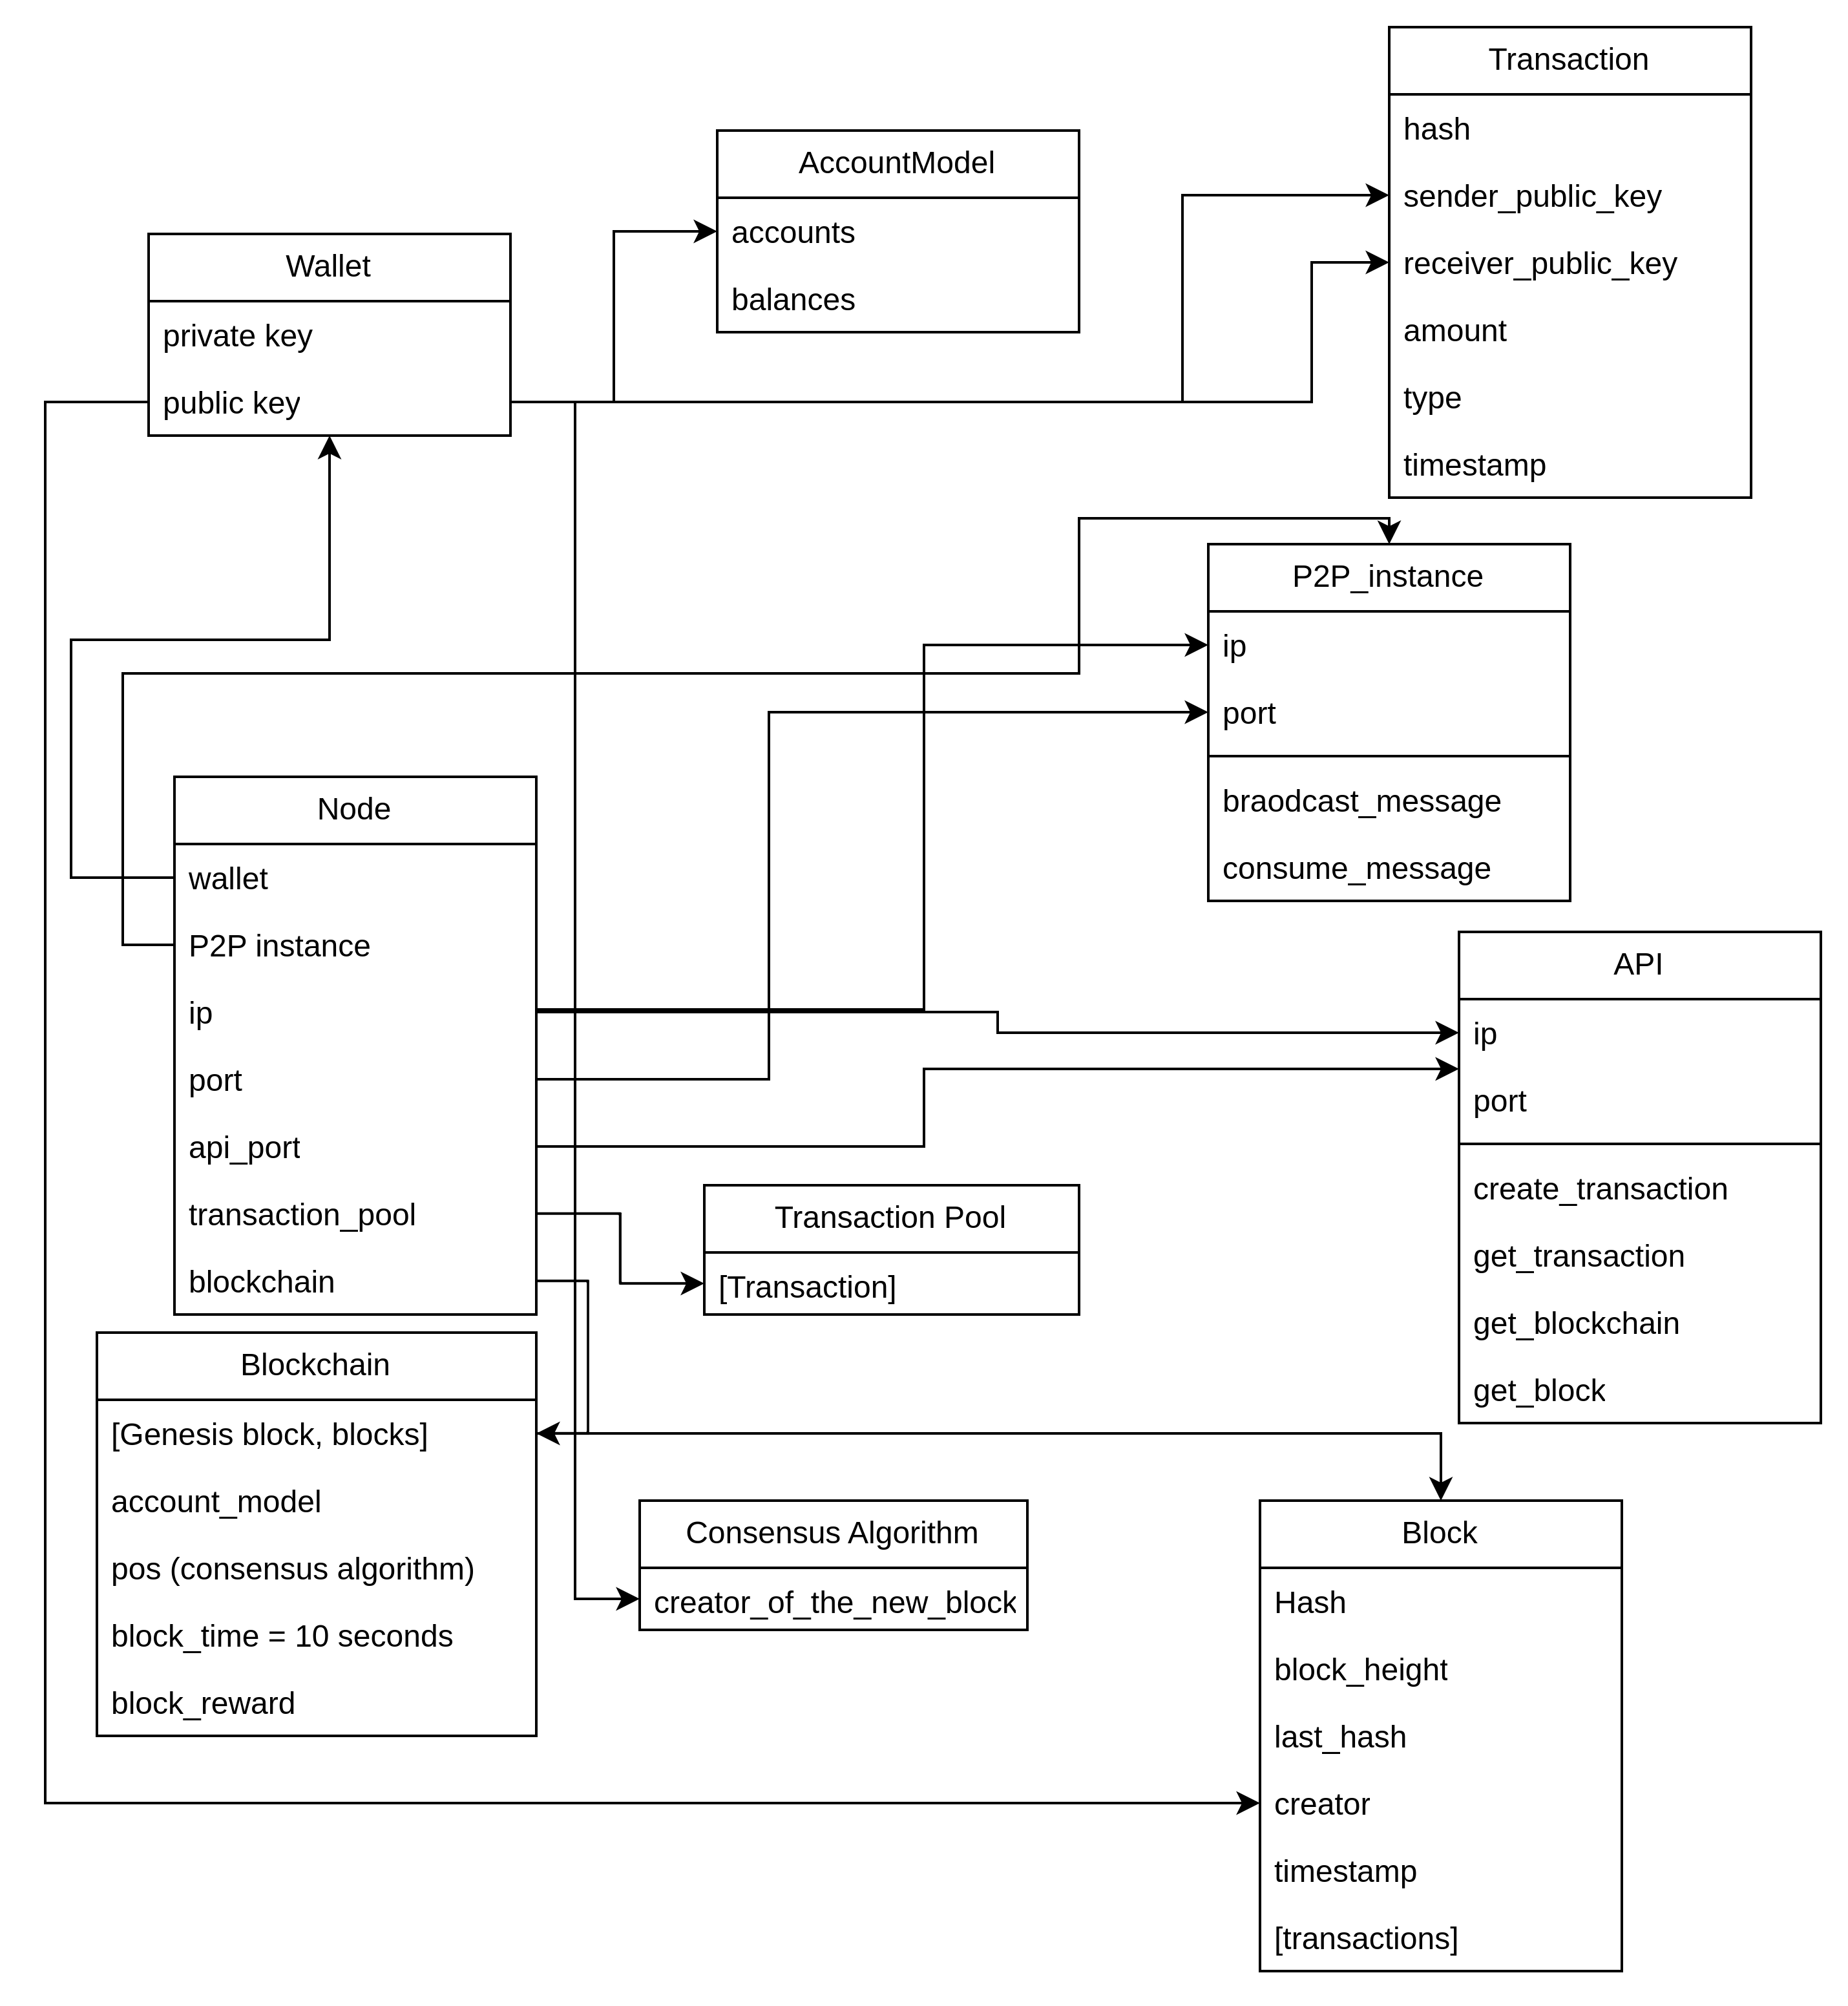
\includegraphics[width=0.9\textwidth]{figures/blockchain_class_diagram.png}
    \caption{UML Class Diagram showing the relationship between Node, Blockchain, and Consensus Strategy.}
    \label{fig:class_diagram}
\end{figure}

Key relationships include:
\begin{itemize}
    \item \textbf{Composition:} The `Node` class owns a `Blockchain` instance and a `TransactionPool`.
    \item \textbf{Aggregation:} The `Blockchain` contains a list of `Block` objects.
    \item \textbf{Polymorphism:} The `Blockchain` relies on the `Consensus` abstract base class, which is implemented by concrete classes like `ProofOfStake` and `ProofOfWork`.
\end{itemize}

\subsection{Data Flow and Transaction Lifecycle}
Understanding how data moves through the system is critical for the "Performance Analysis" module. The lifecycle of a transaction follows the flow illustrated in Figure \ref{fig:tx_flow}.

\begin{figure}[h]
    \centering
    % Placeholder for Flow Chart
    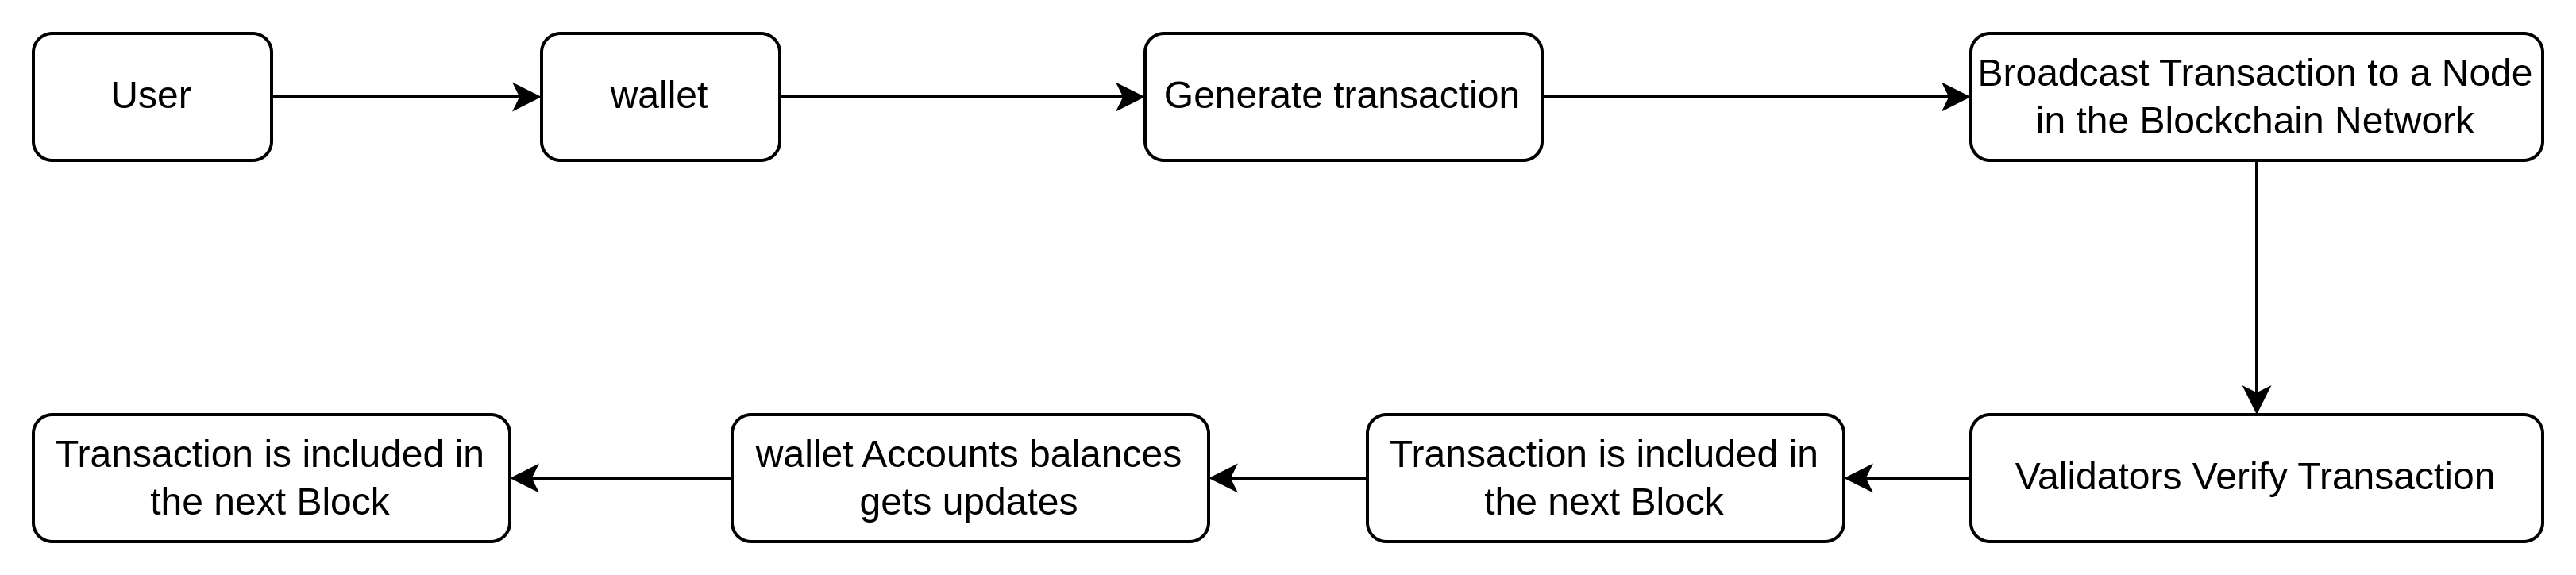
\includegraphics[width=0.7\textwidth]{figures/transaction_lifecycle.png}
    \caption{Data Flow Diagram: Lifecycle of a Transaction from Client to Finalized Block.}
    \label{fig:tx_flow}
\end{figure}



The flow proceeds as follows:
\begin{enumerate}
    \item \textbf{Creation:} A client signs a transaction using their private key (Elliptic Curve Cryptography).
    \item \textbf{Propagation:} The transaction is sent to the Node API and broadcast to the P2P network.
    \item \textbf{Pooling:} Valid transactions are stored in the `TransactionPool` (Mempool).
    \item \textbf{Packaging:} The Consensus engine selects transactions from the pool to create a candidate block.
    \item \textbf{Finalization:} Once the block is mined/validated, it is appended to the chain, and the transactions are removed from the pool.
\end{enumerate}

\section{Technology Stack Justification} \label{ch3_tech_stack}

\subsection{Python as the Core Language}
Python was selected as the implementation language primarily for its dominance in the data science and educational sectors. Unlike C++ (used in Bitcoin), which requires complex memory management, Python allows students to focus on the \textit{logic} of consensus algorithms rather than syntax errors. Libraries such as `pydantic` are used for data validation, enforcing strict typing similar to statically typed languages \cite{van1995python}.

\subsection{Docker for Environment Isolation}
To simulate a distributed network on a single machine, **Docker** containers are used. Each node runs in its own isolated container with a unique IP address within the Docker virtual network. This allows students to simulate network partitions and latency without requiring physical hardware clusters.

\section{Summary}
This chapter defined the architectural blueprint of the educational blockchain. By utilizing a modular, layered architecture and the Strategy Pattern, the system meets the Requirement Analysis for an extensible and clear learning platform. This design sets the stage for the detailed implementation discussed in Chapter \ref{ch4_implementation} and the curriculum exercises in Chapter \ref{ch5_curriculum}.